\documentclass{scrartcl}
\usepackage[utf8]{inputenc}
\usepackage{tikz}
\pagestyle{empty}
\begin{document}
\subsubsection*{Allgemeiner Entscheidungsbaum}
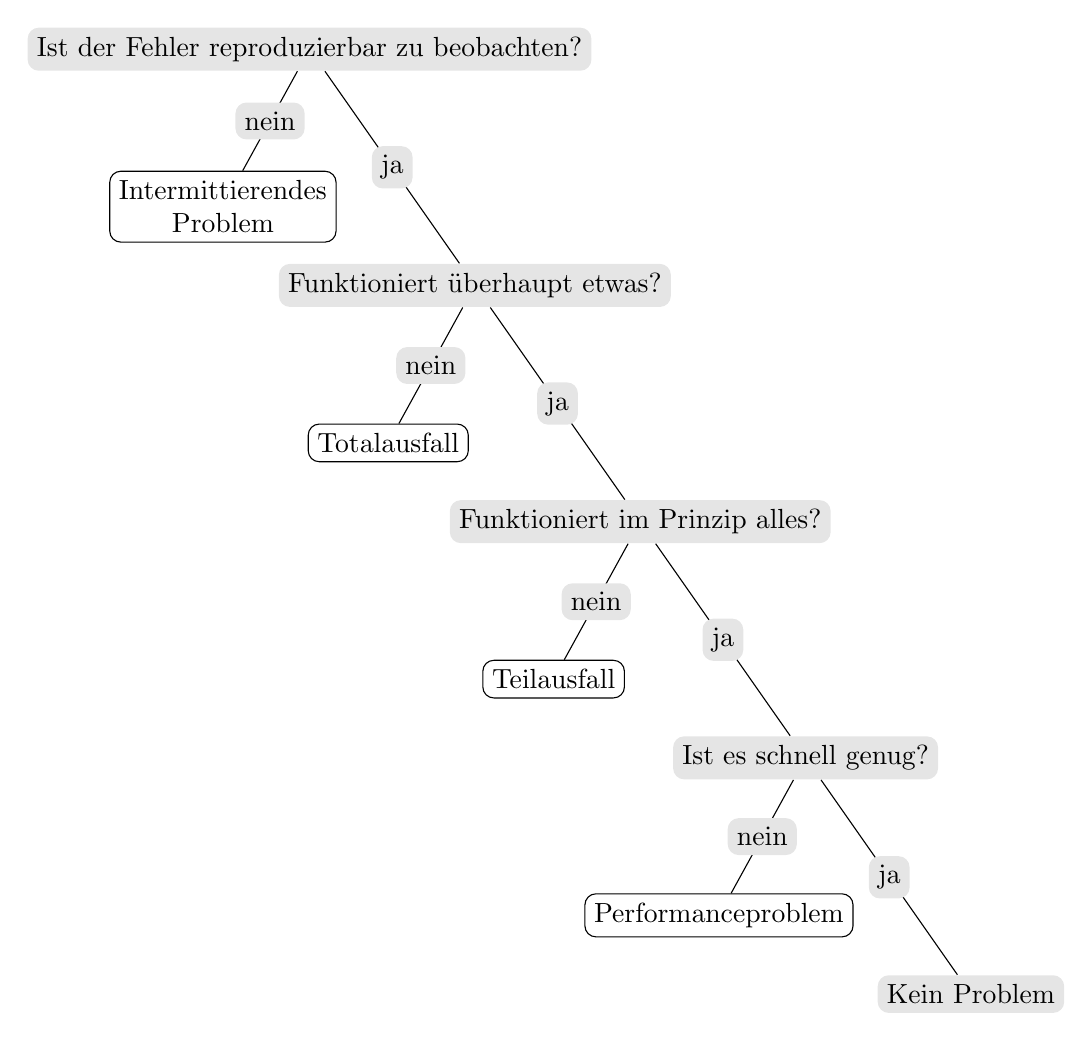
\begin{tikzpicture}
[every node/.style={fill=black!10,rounded corners,align=center},
grow=south, level distance=2cm,
level 1/.style={sibling distance=2.2cm},
level 2/.style={sibling distance=2.2cm},
]
\node{Ist der Fehler reproduzierbar zu beobachten?}
  child{node[draw,fill=white]{Intermittierendes\\Problem}
  edge from parent node[fill=black!10]{nein}}
  child{node at +(1,-1) {Funktioniert überhaupt etwas?}
    child{node[draw,fill=white]{Totalausfall} edge from parent node{nein}}
    child{node at +(1,-1) {Funktioniert im Prinzip alles?}
      child{node[draw,fill=white]{Teilausfall} edge from parent node{nein}}
      child{node at +(1,-1) {Ist es schnell genug?}
        child{node[draw,fill=white]{Performanceproblem}
        edge from parent node{nein}}
        child{node at +(1,-1) {Kein Problem}
        edge from parent node{ja}}
      edge from parent node{ja}}
    edge from parent node{ja}}
  edge from parent node{ja}};
\end{tikzpicture}
\end{document}
